\newcommand{\examplescenescbar}{
	\begin{tikzpicture}[inner sep=0]
	\node(cbar){
\includegraphics[height=\size, width=2mm]{images/examples/inferno}};
	\node[xshift=1mm, anchor=north] at (cbar.north east){\tiny 1};
	\node[xshift=1mm, anchor=south] at (cbar.south east){\tiny 0};
	\end{tikzpicture}
}


% for text extending below like p, q, g
%\tikzset{
%	mylabel2/.style={
%		label={
%			[label distance=-1.25em, anchor=base]north:
%			\fcolorbox{black}{black}{
%				\scriptsize \color{tumgraylight} #1
%			}
%		}
%	}
%}


\begin{tikzpicture}
\tikzset{
	collabel/.style={
		label={
			[label distance=1.5em, anchor=base]south:
			\tiny \color{black} #1
		}
	}
}

\setlength{\fboxsep}{1pt}
\tikzset{
	inlabel/.style={
		label={
			[label distance=-1em, anchor=base]north:
			\fcolorbox{black}{black}{
				\scriptsize \color{tumgraylight} #1
			}
		}
	}
}

\tikzset{
	rowlabel/.style={
		label={
			[label distance=.51em, anchor=north west]north west:
			\fcolorbox{white}{white}{
				\color{black} \textbf{#1}
			}
		}
	}
}

\def\size{1.7cm}
\def\colsize{7mm}

\colsize
\small

\matrix (m) [matrix of nodes, ampersand replacement=\&, row sep=0pt, column sep=2mm]{
	$\V{x}_{RGB,t}$ \& labels $\V{y}$ \& pred. $\hat{\V{y}}$ \& loss $H(\V{y},\hat{\V{y}}$) \& activation \& activation \& activation \& activation
	\\ %% good classificaiton example
	\node[rowlabel=A,inner sep=0]{
\includegraphics[width=\size]{images/examples/16494/rgb}}; \&
	\node[inner sep=0]{
\includegraphics[width=\size]{images/examples/16494/ground_truth}}; \&
	\node[inner sep=0]{
\includegraphics[width=\size]{images/examples/16494/prediction}}; \&
	\node[inner sep=0]{
\includegraphics[width=\size]{images/examples/16494/masked_loss}}; \&
	\node[inlabel=maize,inner sep=0]{
\includegraphics[width=\size]{images/examples/16494/maize}}; \&
	\node[inlabel=meadow,inner sep=0]{
\includegraphics[width=\size]{images/examples/16494/meadow}}; \&
	\node[inlabel=peas,inner sep=0]{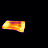
\includegraphics[width=\size]{images/examples/16494/peas}}; \&
	\node[inlabel=rape,inner sep=0]{
\includegraphics[width=\size]{images/examples/16494/rape}}; \&
	\examplescenescbar 
	\\ %% Good example with correct prediction, but some loss
	\node[rowlabel=B,inner sep=0]{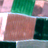
\includegraphics[width=\size]{images/examples/8133/rgb}}; \&
	\node[inner sep=0]{
\includegraphics[width=\size]{images/examples/8133/ground_truth}}; \&
	\node[inner sep=0]{
\includegraphics[width=\size]{images/examples/8133/prediction}}; \&
	\node[inner sep=0]{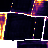
\includegraphics[width=\size]{images/examples/8133/masked_loss}}; \&
	\node[inlabel=spelt,inner sep=0]{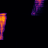
\includegraphics[width=\size]{images/examples/8133/winter_spelt}}; \&
	\node[inlabel=wheat,inner sep=0]{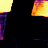
\includegraphics[width=\size]{images/examples/8133/winter_wheat}}; \&
	\node[inlabel=s. barley,inner sep=0]{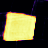
\includegraphics[width=\size]{images/examples/8133/summer_barley}}; \&
	\node[inlabel=maize,inner sep=0]{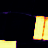
\includegraphics[width=\size]{images/examples/8133/maize}}; \&
	\examplescenescbar 
	\\ %% Good example, only one small field partly wrong classified
	\node[rowlabel=C,inner sep=0]{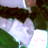
\includegraphics[width=\size]{images/examples/1823/rgb}}; \&
	\node[inner sep=0]{
\includegraphics[width=\size]{images/examples/1823/ground_truth}}; \&
	\node[inner sep=0]{
\includegraphics[width=\size]{images/examples/1823/prediction}}; \&
	\node[inner sep=0]{
\includegraphics[width=\size]{images/examples/1823/masked_loss}}; \&
	\node[inlabel=meadow,inner sep=0]{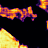
\includegraphics[width=\size]{images/examples/1823/meadow}}; \&
	\node[inlabel=wheat,inner sep=0]{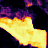
\includegraphics[width=\size]{images/examples/1823/winter_wheat}}; \&
	\node[inlabel=oat,inner sep=0]{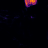
\includegraphics[width=\size]{images/examples/1823/summer_oat}}; \&
	\node[inlabel=maize,inner sep=0]{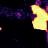
\includegraphics[width=\size]{images/examples/1823/maize}}; \&
	\examplescenescbar 
	\\ %% narrow fields
	\node[rowlabel=D,inner sep=0]{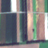
\includegraphics[width=\size]{images/examples/12894/rgb}}; \&
	\node[inner sep=0]{
\includegraphics[width=\size]{images/examples/12894/ground_truth}}; \&
	\node[inner sep=0]{
\includegraphics[width=\size]{images/examples/12894/prediction}}; \&
	\node[inner sep=0]{
\includegraphics[width=\size]{images/examples/12894/masked_loss}}; \&
	\node[inlabel=meadow,inner sep=0]{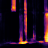
\includegraphics[width=\size]{images/examples/12894/meadow}}; \&
	\node[inlabel=wheat,inner sep=0]{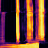
\includegraphics[width=\size]{images/examples/12894/winter_wheat}}; \&
	\node[inlabel=potato,inner sep=0]{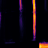
\includegraphics[width=\size]{images/examples/12894/potatoe}}; \&
	\node[inlabel=maize,inner sep=0]{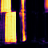
\includegraphics[width=\size]{images/examples/12894/maize}}; \&
	\examplescenescbar 
%	\\ %% Good example, only one small field partly wrong classified
%	\node[rowlabel=D,inner sep=0]{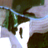
\includegraphics[width=\size]{images/examples/2550/rgb}}; \&
%	\node[inner sep=0]{
\includegraphics[width=\size]{images/examples/2550/ground_truth}}; \&
%	\node[inner sep=0]{
\includegraphics[width=\size]{images/examples/2550/prediction}}; \&
%	\node[inner sep=0]{
\includegraphics[width=\size]{images/examples/2550/masked_loss}}; \&
%	\node[inlabel=maize,inner sep=0]{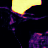
\includegraphics[width=\size]{images/examples/2550/maize}}; \&
%	\node[inlabel=wheat,inner sep=0]{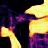
\includegraphics[width=\size]{images/examples/2550/winter_wheat}}; \&
%	\node[inlabel=s. barley,inner sep=0]{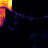
\includegraphics[width=\size]{images/examples/2550/summer_barley}}; \&
%	\node[inlabel=w. barley,inner sep=0]{
\includegraphics[width=\size]{images/examples/2550/winter_barley}}; \&
%	\examplescenescbar 
%	\\ %% Exampe of a forrest, which us a unknown class!
%	\node[rowlabel=D,inner sep=0]{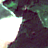
\includegraphics[width=\size]{images/examples/2554/rgb}}; \&
%	\node[inner sep=0]{
\includegraphics[width=\size]{images/examples/2554/ground_truth}}; \&
%	\node[inner sep=0]{
\includegraphics[width=\size]{images/examples/2554/prediction}}; \&
%	\node[inner sep=0]{
\includegraphics[width=\size]{images/examples/2554/masked_loss}}; \&
%	\node[inlabel=maize,inner sep=0]{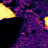
\includegraphics[width=\size]{images/examples/2554/maize}}; \&
%	\node[inlabel=wheat,inner sep=0]{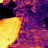
\includegraphics[width=\size]{images/examples/2554/winter_wheat}}; \&
%	\node[inlabel=meadow,inner sep=0]{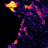
\includegraphics[width=\size]{images/examples/2554/meadow}}; \&
%	\node[inlabel=w. barley,inner sep=0]{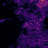
\includegraphics[width=\size]{images/examples/2554/winter_barley}}; \&
%	\examplescenescbar 
%	\\ %% sparse label feature map
%	\node[rowlabel=A,inner sep=0]{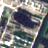
\includegraphics[width=\size]{images/examples/10791/rgb}}; \&
%	\node[inner sep=0]{\includegraphics[width=\size]{images/examples/10791/ground_truth}}; \&
%	\node[inner sep=0]{\includegraphics[width=\size]{images/examples/10791/prediction}}; \&
%	\node[inner sep=0]{\includegraphics[width=\size]{images/examples/10791/masked_loss}}; \&
%	\node[inlabel=maize,inner sep=0]{\includegraphics[width=\size]{images/examples/10791/maize}}; \&
%	\node[inlabel=wheat,inner sep=0]{\includegraphics[width=\size]{images/examples/10791/winter_wheat}}; \&
%	\node[inlabel=meadow,inner sep=0]{\includegraphics[width=\size]{images/examples/10791/meadow}}; \&
%	\node[inlabel=w. barley,inner sep=0]{\includegraphics[width=\size]{images/examples/10791/winter_barley}}; \&
%	\examplescenescbar 
	\\ %% one field completely wrong classified. one field uncertain
	\node[rowlabel=E,inner sep=0]{\includegraphics[width=\size]{images/examples/10792/rgb}}; \&
	\node[inner sep=0]{\includegraphics[width=\size]{images/examples/10792/ground_truth}}; \&
	\node[inner sep=0]{\includegraphics[width=\size]{images/examples/10792/prediction}}; \&
	\node[inner sep=0]{\includegraphics[width=\size]{images/examples/10792/masked_loss}}; \&
	\node[inlabel=rye,inner sep=0]{\includegraphics[width=\size]{images/examples/10792/winter_rye}}; \&
	\node[inlabel=wheat,inner sep=0]{\includegraphics[width=\size]{images/examples/10792/winter_wheat}}; \&
	\node[inlabel=triticale,inner sep=0]{\includegraphics[width=\size]{images/examples/10792/winter_triticale}}; \&
	\node[inlabel=s. barley,inner sep=0]{\includegraphics[width=\size]{images/examples/10792/summer_barley}}; \&
	\examplescenescbar 
	\\ %% Multiple fields uncertain
%	\node[rowlabel=A,inner sep=0]{\includegraphics[width=\size]{images/examples/10879/rgb}}; \&
%	\node[inner sep=0]{\includegraphics[width=\size]{images/examples/10879/ground_truth}}; \&
%	\node[inner sep=0]{\includegraphics[width=\size]{images/examples/10879/prediction}}; \&
%	\node[inner sep=0]{\includegraphics[width=\size]{images/examples/10879/masked_loss}}; \&
%	\node[inlabel=rye,inner sep=0]{\includegraphics[width=\size]{images/examples/10879/winter_rye}}; \&
%	\node[inlabel=triticale,inner sep=0]{\includegraphics[width=\size]{images/examples/10879/winter_triticale}}; \&
%	\node[inlabel=s. barley,inner sep=0]{\includegraphics[width=\size]{images/examples/10879/summer_barley}}; \&
%	\node[inlabel=w. barley,inner sep=0]{\includegraphics[width=\size]{images/examples/10879/winter_barley}}; \&
%	\examplescenescbar 
%	\\ %% one field uncertain
%	\node[rowlabel=A,inner sep=0]{\includegraphics[width=\size]{images/examples/10969/rgb}}; \&
%	\node[inner sep=0]{\includegraphics[width=\size]{images/examples/10969/ground_truth}}; \&
%	\node[inner sep=0]{\includegraphics[width=\size]{images/examples/10969/prediction}}; \&
%	\node[inner sep=0]{\includegraphics[width=\size]{images/examples/10969/masked_loss}}; \&
%	\node[inlabel=wheat,inner sep=0]{\includegraphics[width=\size]{images/examples/10969/winter_wheat}}; \&
%	\node[inlabel=triticale,inner sep=0]{\includegraphics[width=\size]{images/examples/10969/winter_triticale}}; \&
%	\node[inlabel=rye,inner sep=0]{\includegraphics[width=\size]{images/examples/10969/winter_rye}}; \&
%	\node[inlabel=rape,inner sep=0]{\includegraphics[width=\size]{images/examples/10969/rape}}; \&
%	\examplescenescbar 
	\\ %% very bad classification
	\node[rowlabel=F,inner sep=0]{\includegraphics[width=\size]{images/examples/172/rgb}}; \&
	\node[inner sep=0]{\includegraphics[width=\size]{images/examples/172/ground_truth}}; \&
	\node[inner sep=0]{\includegraphics[width=\size]{images/examples/172/prediction}}; \&
	\node[inner sep=0]{\includegraphics[width=\size]{images/examples/172/masked_loss}}; \&
	\node[inlabel=wheat,inner sep=0]{\includegraphics[width=\size]{images/examples/172/winter_wheat}}; \&
	\node[inlabel=meadow,inner sep=0]{\includegraphics[width=\size]{images/examples/172/meadow}}; \&
	\node[inlabel=maize,inner sep=0]{\includegraphics[width=\size]{images/examples/172/maize}}; \&
	\node[inlabel=w.barley,inner sep=0]{\includegraphics[width=\size]{images/examples/172/winter_barley}}; \&
	\examplescenescbar 
	\\
};

%\tiny
%%\node[inner sep=0]{\includegraphics[width=\size]{images/examples/color__asparagus}};
%\matrix (n) [matrix of nodes, ampersand replacement=\&, row sep=0pt, column sep=2mm, below= 0mmof m]{
%	\node[collabel=asparag., inner sep=0]{\includegraphics[width=\colsize]{images/examples/color__asparagus}}; \&
%	\node[collabel=bean,inner sep=0]{\includegraphics[width=\colsize]{images/examples/color__beans}}; \&
%	\node[collabel=hop,inner sep=0]{\includegraphics[width=\colsize]{images/examples/color__hop}}; \&
%	\node[collabel=maize,inner sep=0]{\includegraphics[width=\colsize]{images/examples/color__maize}}; \&
%	\node[collabel=meadow,inner sep=0]{\includegraphics[width=\colsize]{images/examples/color__meadow}}; \&
%	\node[collabel=peas,inner sep=0]{\includegraphics[width=\colsize]{images/examples/color__peas}}; \&
%	\node[collabel=potato,inner sep=0]{\includegraphics[width=\colsize]{images/examples/color__potatoe}}; \&
%	\node[collabel=rape,inner sep=0]{\includegraphics[width=\colsize]{images/examples/color__rape}}; \&
%	\node[collabel=soybean,inner sep=0]{\includegraphics[width=\colsize]{images/examples/color__soybeans}}; \&
%	\node[collabel=beet,inner sep=0]{\includegraphics[width=\colsize]{images/examples/color__sugar_beet}}; \&
%	\node[collabel=s. barley,inner sep=0]{\includegraphics[width=\colsize]{images/examples/color__summer_barley}}; \&
%	\node[collabel=oat,inner sep=0]{\includegraphics[width=\colsize]{images/examples/color__summer_oat}}; \&
%	\node[collabel=w. barley,inner sep=0]{\includegraphics[width=\colsize]{images/examples/color__winter_barley}}; \&
%	\node[collabel=rye,inner sep=0]{\includegraphics[width=\colsize]{images/examples/color__winter_rye}}; \&
%	\node[collabel=spelt,inner sep=0]{\includegraphics[width=\colsize]{images/examples/color__winter_spelt}}; \&
%	\node[collabel=triticale,inner sep=0]{\includegraphics[width=\colsize]{images/examples/color__winter_triticale}}; \&
%	\node[collabel=wheat,inner sep=0]{\includegraphics[width=\colsize]{images/examples/color__winter_wheat}}; \&
%	\\
%};
\end{tikzpicture}